% ---- pg-232 （书页 220） ----
\[
\left(\frac{1}{n_1}+\frac{1}{n_2}\right)c^2=\left(\frac{1}{50}+\frac{1}{50}\right)\times\frac{98\times 2}{97}\times F_{2,97}(0.05)=0.25
\]
由结论 6.2 知置信椭圆的主轴沿特征向量 $\mathbf{e}_i$ 的长度为
\[
\sqrt{\lambda_i}\sqrt{\left(\frac{1}{n_1}+\frac{1}{n_2}\right)c^2}=\sqrt{\lambda_i}\times\sqrt{0.25}
\]
即在 $\mathbf{e}_1$ 方向上长度为 1.15 个单位，在 $\mathbf{e}_2$ 方向上长度为 0.65 个单位. 95\% 置信椭圆图示于\hyperref[fig:6.1]{图 6.1}. $\boldsymbol{\mu}_1-\boldsymbol{\mu}_2=\mathbf{0}$ 显然不在此椭圆内，因而我们得出结论：两种制皂工艺有差别. 从图可看出，虽然两种工艺生产的肥皂具有相同的舒适度（$X_2$），但第二种工艺生产的肥皂的泡沫量（$X_1$）较多.\hfill$\blacksquare$

\begin{mvfigure}
\centering
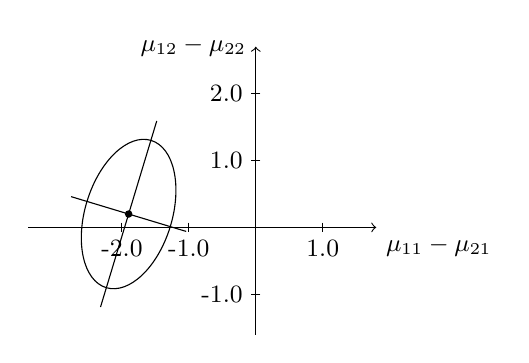
\begin{tikzpicture}[scale=0.85,every node/.style={font=\small}]
% 坐标轴
\draw[->] (-3.4,0)--(1.8,0) node[below right] {$\mu_{11}-\mu_{21}$};
\draw[->] (0,-1.6)--(0,2.7) node[left] {$\mu_{12}-\mu_{22}$};
% 刻度
\foreach \x/\lab in {-2.0/-2.0,-1.0/-1.0,1.0/1.0} {
  \draw (\x,0.07)--(\x,-0.07);
  \node[below] at (\x,-0.05) {\lab};
}
\foreach \y/\lab in {-1.0/-1.0,1.0/1.0,2.0/2.0} {
  \draw (0.07,\y)--(-0.07,\y);
  \node[left] at (-0.05,\y) {\lab};
}
% 95% 置信椭圆
\draw[rotate around={73:(-1.9,0.2)}] (-1.9,0.2) ellipse ({1.15} and {0.65});
% 主轴方向
\draw (-2.32,-1.19)--(-1.48,1.59);
\draw (-2.76,0.46)--(-1.04,-0.06);
\fill (-1.9,0.2) circle (1.6pt);
\end{tikzpicture}
\phantomsection\label{fig:6.1}\mvcap{图 6.1\quad $\boldsymbol{\mu}_1-\boldsymbol{\mu}_2$ 的 95\% 置信椭圆}
\end{mvfigure}

\subsection{联合置信区间}

有可能推出向量 $\boldsymbol{\mu}_1-\boldsymbol{\mu}_2$ 诸分量的联合置信区间，只要考虑诸均值向量之差的所有可能的线性组合即可. 假定各个多元母总体均服从多元正态分布，且具有公共的协方差矩阵 $\boldsymbol{\Sigma}$.

\mvthm{结论 6.3}{设 $c^2=[(n_1+n_2-2)p/(n_1+n_2-p-1)]F_{p,n_1+n_2-p-1}(\alpha)$. 此时对任意的 $\boldsymbol{a}$，
\[
\boldsymbol{a}'(\bar{\mathbf{X}}_1-\bar{\mathbf{X}}_2)\pm c\sqrt{\boldsymbol{a}'\left(\frac{1}{n_1}+\frac{1}{n_2}\right)\mathbf{S}_p\boldsymbol{a}}
\]
将以概率 $1-\alpha$ 包含 $\boldsymbol{a}'(\boldsymbol{\mu}_1-\boldsymbol{\mu}_2)$. 特别是
\[
(\bar{X}_{1i}-\bar{X}_{2i})\pm c\sqrt{\left(\frac{1}{n_1}+\frac{1}{n_2}\right)s_{ii,\mathrm{p}}},\quad i=1,2,\cdots,p
\]
将包含 $\mu_{1i}-\mu_{2i}$.}

\mvbold{证明}\quad 考虑由观测值 $X_{11},X_{12},\cdots,X_{1n_1}$ 与 $X_{21},X_{22},\cdots,X_{2n_2}$ 构成的一元线性组合
\[
\boldsymbol{a}'\mathbf{X}_{1j}=a_1X_{1j1}+a_2X_{1j2}+\cdots+a_pX_{1jp}\qquad 及\qquad \boldsymbol{a}'\mathbf{X}_{2j}=a_1X_{2j1}+a_2X_{2j2}+\cdots+a_pX_{2jp}
\]
这些线性组合的样本均值与样本方差分别为 $\boldsymbol{a}'\bar{\mathbf{X}}_1$，$\boldsymbol{a}'\mathbf{S}_1\boldsymbol{a}$ 及 $\boldsymbol{a}'\bar{\mathbf{X}}_2$，$\boldsymbol{a}'\mathbf{S}_2\boldsymbol{a}$，其中 $\bar{\mathbf{X}}_1,\mathbf{S}_1$ 与 $\bar{\mathbf{X}}_2,\mathbf{S}_2$ 分别为原样本的样本均值和样本方差（见结论 3.5）. 当两个母总体具有相同的协方差阵时，$s_{1,a}^2=\boldsymbol{a}'\mathbf{S}_1\boldsymbol{a}$ 与 $s_{2,a}^2=\boldsymbol{a}'\mathbf{S}_2\boldsymbol{a}$ 二者均为线性组合 $\boldsymbol{a}'\mathbf{X}_1$ 与 $\boldsymbol{a}'\mathbf{X}_2$ 的公共总体方差 $\boldsymbol{a}'\boldsymbol{\Sigma}\boldsymbol{a}$ 的估计量. 融合这些估计量，便得
\phantomsection\label{eq:6-25}
\begin{equation}
\begin{aligned}
s_{a,\mathrm{p}}^2&=\frac{(n_1-1)s_{1,a}^2+(n_2-1)s_{2,a}^2}{(n_1+n_2-2)}\\
&=\boldsymbol{a}'\left[\frac{n_1-1}{n_1+n_2-2}\mathbf{S}_1+\frac{n_2-1}{n_1+n_2-2}\mathbf{S}_2\right]\boldsymbol{a}\\
&=\boldsymbol{a}'\mathbf{S}_p\boldsymbol{a}
\end{aligned}
\tag{6-25}
\end{equation}
为了根据 $\boldsymbol{a}'\mathbf{X}_{1j}$ 和 $\boldsymbol{a}'\mathbf{X}_{2j}$ 检验 $H_0: \boldsymbol{a}'(\boldsymbol{\mu}_1-\boldsymbol{\mu}_2)=\boldsymbol{a}'\boldsymbol{\delta}_0$，我们构造一元二样本 $t$ 统计量的平方
\phantomsection\label{eq:6-26}
\begin{equation}
t_a^2=\frac{[\boldsymbol{a}'(\bar{\mathbf{X}}_1-\bar{\mathbf{X}}_2)-\boldsymbol{a}'(\boldsymbol{\mu}_1-\boldsymbol{\mu}_2)]^2}{\left(\frac{1}{n_1}+\frac{1}{n_2}\right)s_{a,\mathrm{p}}^2}=\frac{[\boldsymbol{a}'(\bar{\mathbf{X}}_1-\bar{\mathbf{X}}_2-(\boldsymbol{\mu}_1-\boldsymbol{\mu}_2))]^2}{\boldsymbol{a}'\left(\frac{1}{n_1}+\frac{1}{n_2}\right)\mathbf{S}_p\boldsymbol{a}}
\tag{6-26}
\end{equation}
根据\hyperref[eq:2-50]{式(2-50)}中的最大化引理，其中 $\boldsymbol{d}=(\bar{\mathbf{X}}_1-\bar{\mathbf{X}}_2-(\boldsymbol{\mu}_1-\boldsymbol{\mu}_2))$ 和 $\mathbf{B}=(1/n_1+1/n_2)\mathbf{S}_p$，我们有，对一切 $\boldsymbol{a}\neq\mathbf{0}$
\[
\begin{aligned}
t_a^2&\leqslant (\bar{\mathbf{X}}_1-\bar{\mathbf{X}}_2-(\boldsymbol{\mu}_1-\boldsymbol{\mu}_2))'\left[\left(\frac{1}{n_1}+\frac{1}{n_2}\right)\mathbf{S}_p\right]^{-1}(\bar{\mathbf{X}}_1-\bar{\mathbf{X}}_2-(\boldsymbol{\mu}_1-\boldsymbol{\mu}_2))\\
&=T^2
\end{aligned}
\]
